\section{Specific Requirements}
\subsection{External Interface Requirements}
\subsubsection{User Interfaces}
	\paragraph{Home Page - Mobile Application}
	\begin{figure}[!h]
		\begin{center}					
			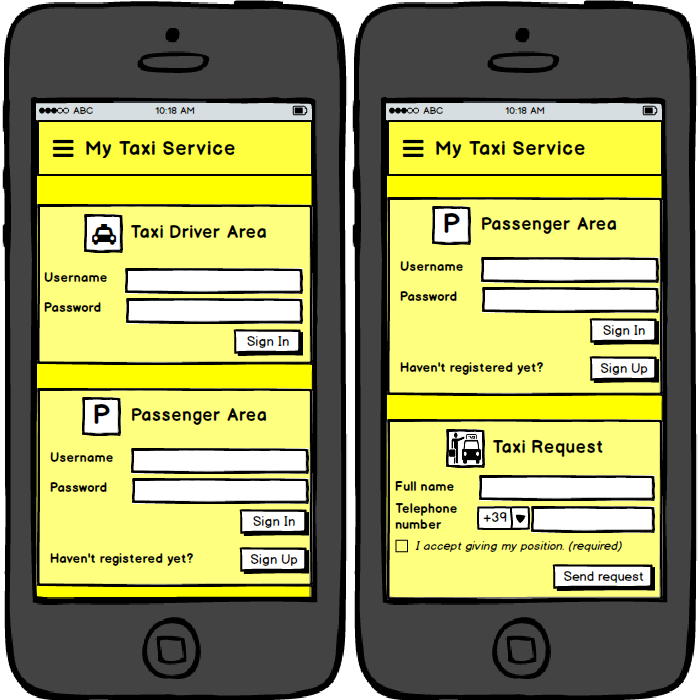
\includegraphics[scale=0.5]{../SE2_MOCKUPS/MobileAppHomePage.png}
			\caption{Home Page - Mobile Application}
		\end{center}	
	\end{figure}

\newpage
\paragraph{Home Page - Web Application}
\begin{figure}[!h]
	\begin{center}					
		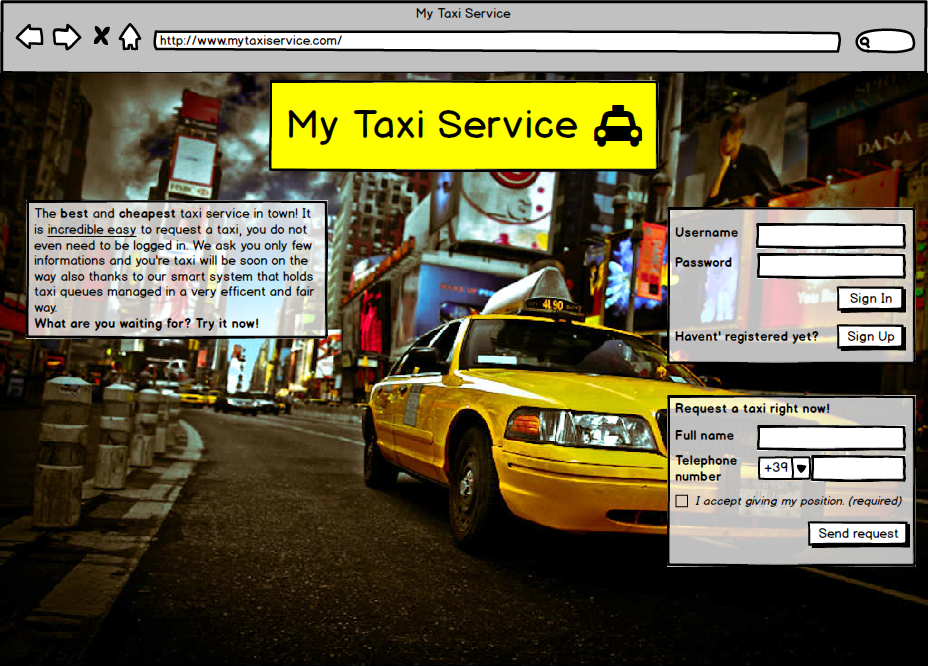
\includegraphics[scale=0.45]{../SE2_MOCKUPS/WebAppHomePage.png}
		\caption{Home Page - Web Application}
	\end{center}	
\end{figure}
\newpage
\paragraph{Registration Form - Mobile Application}
\begin{figure}[!h]
	\begin{center}
		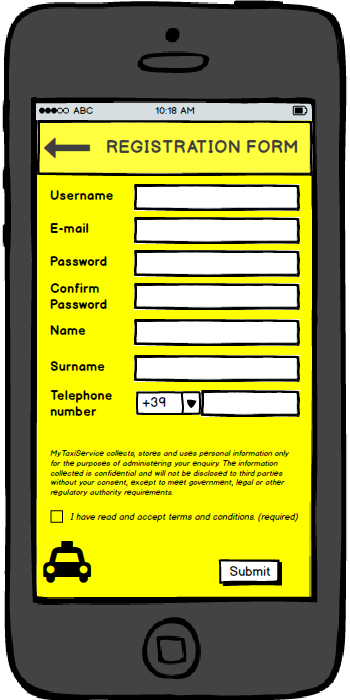
\includegraphics[scale=0.5]{../SE2_MOCKUPS/MobileAppRegistrationForm.png}
		\caption{Registration Form - Mobile Application}	
	\end{center}
\end{figure}
\newpage
\paragraph{Registration Form - Web Application}
\begin{figure}[!h]
	\begin{center}
		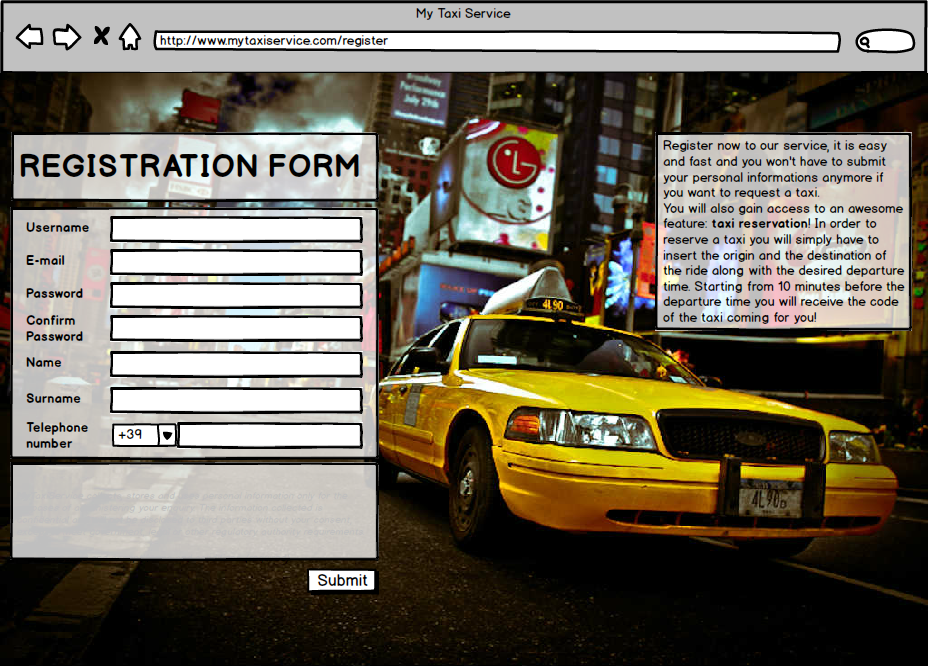
\includegraphics[scale=0.45]{../SE2_MOCKUPS/WebAppRegistrationForm.png}
		\caption{Registration Form -Web Application}	
	\end{center}
\end{figure}
\newpage
\paragraph{Passenger Area - Mobile Application}
\begin{figure}[!h]
	\begin{center}
		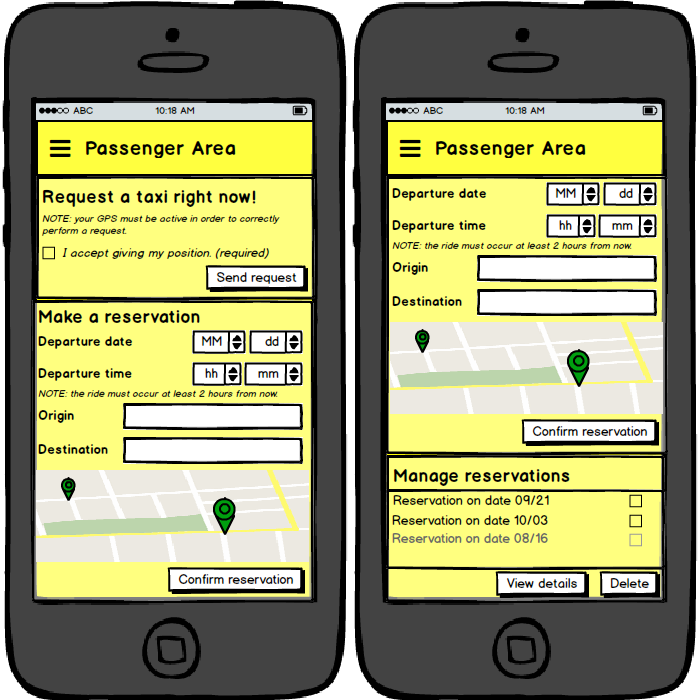
\includegraphics[scale=0.5]{../SE2_MOCKUPS/MobileAppPassengerArea.png}
		\caption{Passenger Area - Mobile Application}
	\end{center}	
\end{figure}
\newpage
\paragraph{Passenger Area - Web Application}
\begin{figure}[!h]
	\begin{center}
		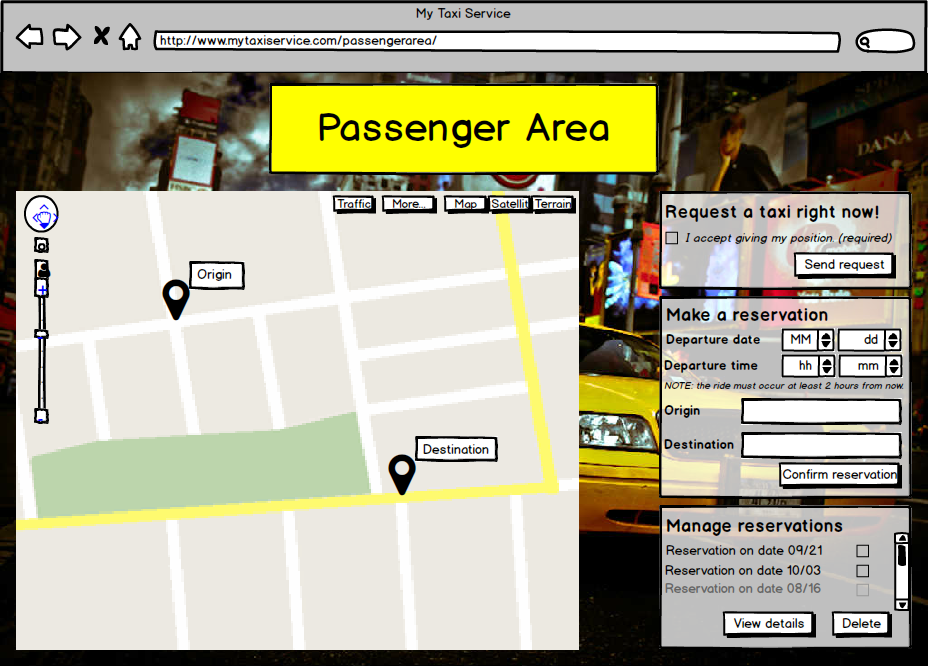
\includegraphics[scale=0.45]{../SE2_MOCKUPS/WebAppPassengerArea.png}
		\caption{Passenger Area - Web Application}
	\end{center}	
\end{figure}
\newpage
\paragraph{Request Confirmation - Mobile Application}
\begin{figure}[!h]
	\begin{center}
		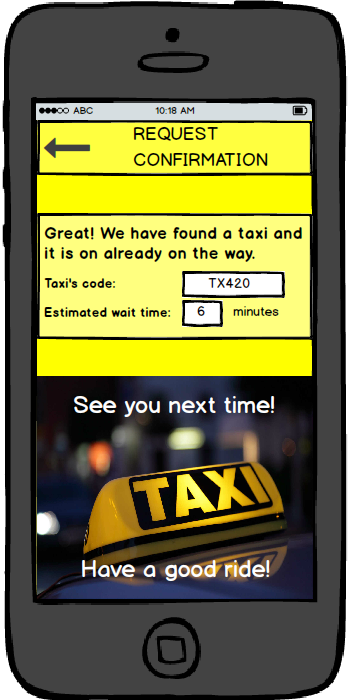
\includegraphics[scale=0.5]{../SE2_MOCKUPS/MobileAppRequestConfirmation.png}
		\caption{Request Confirmation - Mobile Application}
	\end{center}	
\end{figure}
\newpage
\paragraph{Request Confirmation - Web Application}
\begin{figure}[!h]
	\begin{center}
		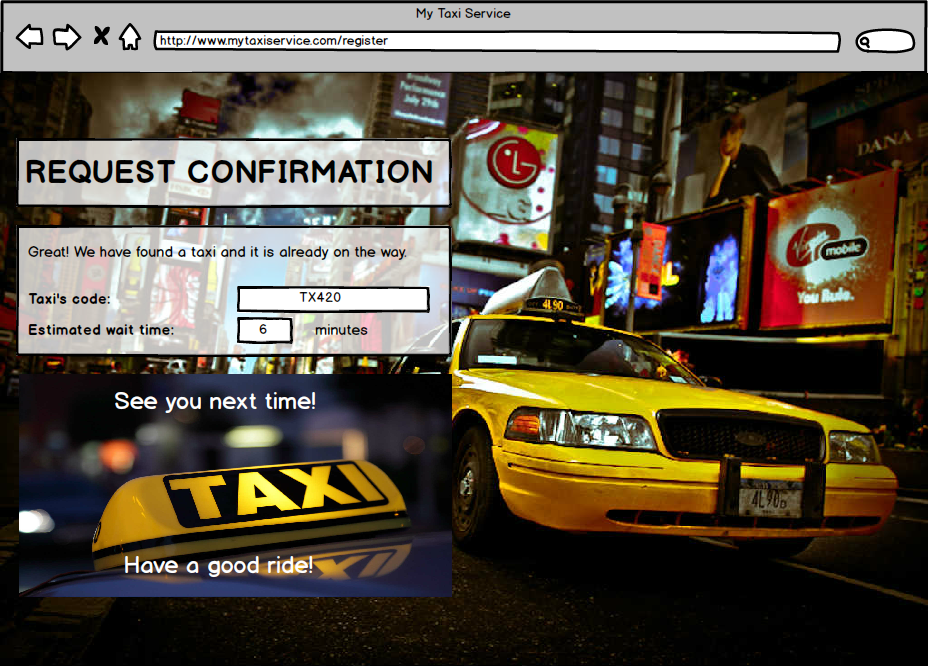
\includegraphics[scale=0.45]{../SE2_MOCKUPS/WebAppRequestConfirmation.png}
		\caption{Request Confirmation - Web Application}
	\end{center}	
\end{figure}
\newpage
\paragraph{Taxi Driver Area - Mobile Application}
\begin{figure}[!h]
	\begin{center}
		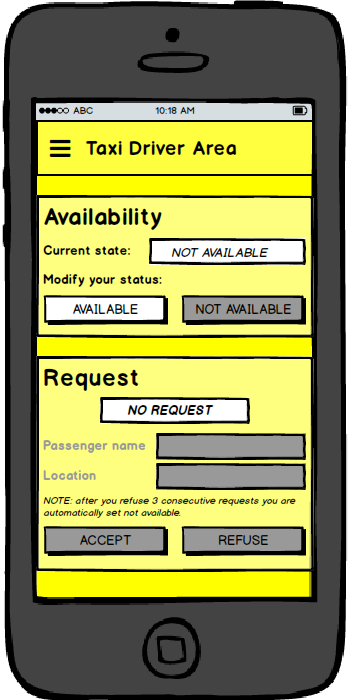
\includegraphics[scale=0.5]{../SE2_MOCKUPS/MobileAppTaxiDriverArea.png}
		\caption{Taxi Driver Area - Mobile Application}	
	\end{center}
\end{figure}
\newpage
\subsubsection{API Interfaces}
For taxi waiting time and other minor features we decided to use Google Maps API.
It is a very powerful library that perfectly fits our needs.
When a taxi accepts a request, the system retrieves its position and, through
those APIs, is able to process either the hypothetical route that the taxi will
follow to reach the passenger's position and, consequently, the arrival time.
The system will, then, forward those information to the passenger.
\subsubsection{Hardware Interfaces}
Our project includes a web and a mobile application, so it does not require
any external hardware interface.
\subsubsection{Software Interfaces}
\begin{itemize}
	\item Database Management System (DBMS):
	\begin{itemize}
		\item Name: MySQL.
		\item Version: 5.6.21
		\item Source: http://www.mysql.it/
	\end{itemize}
	\item Java Virtual Machine (JVM).
	\begin{itemize}
		\item Name: JEE
		\item Version: 7
		\item Source: http://www.oracle.com/technetwork/java/javaee/tech/index.html
	\end{itemize}
	\item Application server:
	\begin{itemize}
		\item Name: Glassfish.
		\item Version: 4.1.
		\item Source: https://glassfish.java.net/
	\end{itemize}
	\item Operating System (OS).
	\begin{itemize}
		\item Application must be able to run on any SO which supports JVM and DBMS specified before.
	\end{itemize}
\end{itemize}
\subsubsection{Communication Interfaces}
\begin{center}
	\begin{tabular}{ | l | l | l | p{5cm} |}
		\hline
		Protocol & Application & Port 	\\ \hline
		TCP & HTTPS & 443				\\ \hline
		TCP & HTTP  & 80				\\ \hline
		TCP & DBMS  & 3306 (default)	\\ \hline
	\end{tabular}
\end{center}
\subsection{Functional Requirements}
\subsubsection{Permit a guest to register to the service}
\begin{enumerate}[label=\bfseries R\arabic*:]
	\item The system shows the registration form to the user when he presses the sign up button.
	\item When the user inserts the username, the email or the phone number, the system verifies that neither of those have already been selected by someone else.
\end{enumerate}
\subsubsection{Permit a guest to request a taxi}
\begin{enumerate}[label=\bfseries R\arabic*:]
	\item The system has to provide a form for storing user basic personal informations.
	\item The system has to ask the user the consensus in order to use his position.
	\item The system has to search for an available taxi in the same area of the user after he presses the request button.
\end{enumerate}
\subsubsection{Permit a guest to sign in}
\begin{enumerate}[label=\bfseries R\arabic*:]
	\item The system has to provide the user a sign in form.
	\item The system, during sign in, verifies that the username and the password inserted by the user have a match in the DB.
\end{enumerate}
\subsubsection{Permit a registered passenger to request a taxi}
\begin{enumerate}[label=\bfseries R\arabic*:]
	\item The system has to ask the user the consensus in order to use his position.
	\item The system has to search for an available taxi in the same area of the user after he presses the request button.
\end{enumerate}
\subsubsection{Permit a registered passenger to make a reservation}
\begin{enumerate}[label=\bfseries R\arabic*:]
	\item User must be already registered and logged in the application.
	\item User must make a reservation at least 2 hours before the request time.
	\item User must provide time, origin and destination of the ride at the moment of the reservation.
	\item User must confirm the reservation process.
	\item The reservation can be deleted by the user himself.
\end{enumerate}
\subsubsection{Permit a registered passenger to cancel a reservation}
\begin{enumerate}[label=\bfseries R\arabic*:]
	\item The system shall check that the passenger is already registered and signed in with
	the correct	credentials.
	\item The system shall check that the request the passenger is deleting, exists and belongs
	to him.
	\item The system shall check that it's not after 10 minutes before the reservation request time.
	\item This process is not reversible
\end{enumerate}
\subsubsection{Permit a taxi driver to give the system his availability}
\begin{enumerate}[label=\bfseries R\arabic*:]
	\item The system shall check that the taxi driver is already registered and signed in with
	the correct	credentials.
	\item The system shall check that the taxi driver is actually unavailable and then
	let the taxi driver set his status as unavailable through the mobile application.
\end{enumerate}
\subsubsection{Permit a taxi driver to revoke his availability}
\begin{enumerate}[label=\bfseries R\arabic*:]
	\item The system shall check that the taxi driver is already registered and signed in with
	the correct	credentials.
	\item The system shall check that the taxi driver is actually available and then
	let the taxi driver set his status as unavailable through the mobile application.
	\item The system shall revoke it automatically if it registers three consecutive request
	rejections.
\end{enumerate}
\subsubsection{Permit a taxi driver to accept a ride request}
\begin{enumerate}[label=\bfseries R\arabic*:]
	\item The system shall check that the taxi driver is already registered and signed in with
	the correct	credentials.
	\item When the system receives a taxi request, it shall remove the first taxi driver
	of that area from the relative queue and notify him, through the mobile application,
	that someone is requesting his taxi.
	\item When the taxi driver receives the notification, he accepts
	\item The system shall register the answer and inform the passenger
	that this taxi is reaching his position.
\end{enumerate}
\subsubsection{Permit a taxi driver to refuse a ride request}
\begin{enumerate}[label=\bfseries R\arabic*:]
	\item The system shall check that the taxi driver is already registered and signed in with
	the correct	credentials.
	\item When the system receives a taxi request, it shall remove the first taxi driver
	of that area from the relative queue and notify him, through the mobile application,
	that someone is requesting his taxi.
	\item When the taxi driver receives the notification, he declines the request.
	\item If this taxi driver is at the third consecutive rejection, the system shall set his status as unavailable,
	notifying him
	\item If this taxi driver is at the first or second consecutive rejection, the system shall put him
	at the end of his area queue.
\end{enumerate}
\subsection{Scenarios}
\subsubsection{Occasional user}
Mario, an important businessman, has just arrived by train in our city for the first time.
His train had technical issues and now he is a bit late for the meeting on 
the opposite side of our town, so he does not want to take public transports.
The best solution is to call a taxi.
He opens the browser on his smartphone and, inserting name and surname, sends a taxi request
to our system. As soon as possible he receives a notification with the taxi ID number and the
waiting time before the taxi arrival. In less than no time he will reach the meeting location.
\subsubsection{Habitual user}
The meeting of Mario went very well: he started an important collaboration with a local
company. He will have to come back often in our town. He found our service very useful, so
he decides to register and download the mobile application. After a couple of weeks he has to
come back. Unfortunately his train had technical issues, and he risks to be late to the
meeting again. This time he has our application installed on his mobile device, so with only
few taps and no additional information provided requests a taxi. As soon as possible he receives
a notification with the taxi ID number and the	waiting time before the taxi arrival.
In less than no time he will reach the meeting location.
\subsubsection{Taxi reservation}
After another couple of weeks, Mario has to come back in our town again. He thinks that he 
will never be so unlucky to find a defective train for the third consecutive time,
so he decides to make a reservation before leaving,	in order to find a taxi waiting for him
at the train station at his arrival. Using the mobile application, he fills in all the
necessary fields, indicating hour and place of the request.
Now he can airily taste	his journey.
\subsubsection{Deleting a taxi reservation}
Mario's train has technical issues. Poor Mario, he's so unlucky! He will be very late, 
so he does not want to let the taxi wait so long. He opens our application and, 30 minutes
before the taxi request, he selects the reservation and deletes it. Once arrived he will
request a taxi as usual.
\subsubsection{Taxi driver}
A taxi driver, Luigi, is having a little break, eating his favourite chocolate bar in his taxi. Suddenly
his phone rings: a notification has just arrived. But he's having a break, so he does not answer.
After 1 minute, the system automatically records a negative answer from the taxi driver.
Luigi slowly ends his bar and starts answering some messages on his smartphone. Suddenly his phone
rings. He sees the notification, but he's very busy, so he declines the request. Luigi greets his
friend on the chat and goes back to work. After a few minutes his phone rings again. A man called
Mario is requesting a taxi in his area, right next to the train station. He accepts the request and
starts driving towards the location of the customer.
\subsubsection{Taxi availability}
After a hard morning, Luigi decides that it is the right time to have lunch. He opens our mobile
application and sets his status as unavailable: he does not want to be disturbed during such an
important moment. After a hearty lunch, he goes back to work, so he picks up his phone, opens our
application and sets his status as available. He works hard for the whole afternoon and, after the
last passenger, he's so tired that he forgets the status on available. The system sends him 1, 2, 3
notifications of requests, but Luigi has a huge headache and can not hear the phone ringing. After
the third request without answer the system automatically sets the driver as unavailable.
Finally Luigi will get its deserved peace.
\newpage
\subsection{UML models}
\subsubsection{Use Case diagram}
\begin{figure}[h!]
	\centering
	\graphicspath{ {../SE2_IMAGES/} }
	\includegraphics[height=0.8\textheight]{UseCase.png}
	\caption{Use Case Diagram for MyTaxiService}
\end{figure}
\newpage
\subsubsection{Class diagram}
\begin{figure}[h!]
	\centering
	\graphicspath{ {../SE2_IMAGES/} }
	\includegraphics[width=\linewidth]{ClassDiagram.png}
	\caption{Class Diagram for MyTaxiService}
\end{figure}
\newpage
\paragraph{Guest Registration}
\begin{center}
	\begin{tabular}{ | l | p{8cm} |}
		\hline
		Actor &  Guest	\\ \hline
		Preconditions & The guest has not registered yet to the service		\\ \hline
		Execution Flow & \begin{enumerate}
			\item The guest presses the sign up button and access the registration form
			\item The form requires to insert username, email, password, password confirmation, name, surname, telephone number and to accept terms and conditions
			\item The system verifies that username, email and telephone number are uniques
			\item The system confirms the registration
			\item The system automatically loads the Passenger Area page
		\end{enumerate}		\\ \hline
		Postconditions & The guest is now a Registered Passenger and is logged in to the service	\\ \hline
		Exceptions & Username, password or email are not uniques; the registration fails \\ \hline
	\end{tabular}
\end{center}
\newpage
\begin{landscape}
\begin{figure}[!h]
	\begin{center}			
		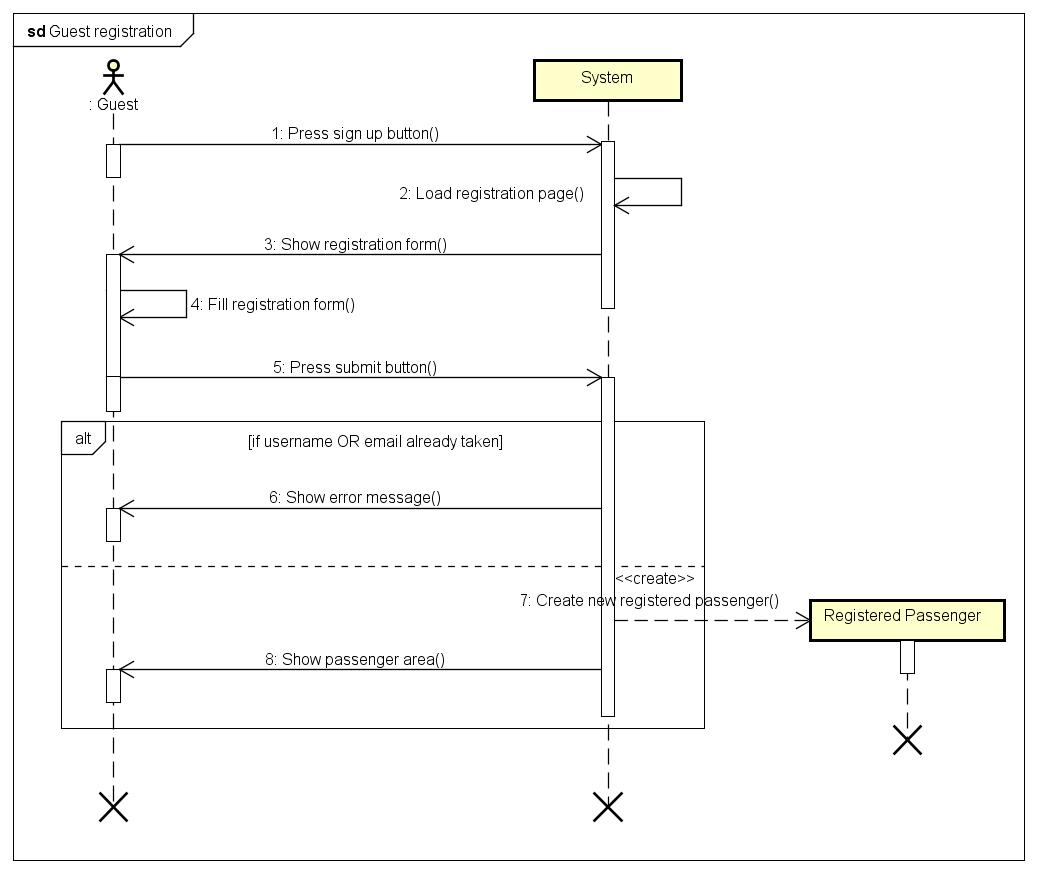
\includegraphics[height=\textheight]{../SE2_SD/GuestRegistration}
		\caption{Sequence Diagram - Guest Registration}	
	\end{center}
\end{figure}
\end{landscape}
\newpage
\paragraph{Registered Passenger Sign In}
\begin{center}
	\begin{tabular}{ | l | p{8cm} |}
		\hline
		Actor &  Registered Passenger	\\ \hline
		Preconditions & The registered passenger is registered to the service	\\ \hline
		Execution Flow & \begin{enumerate}
			\item The registered passenger fills the sign in form, which requires to insert username and password
			\item The guest presses the sign in
			\item The system verifies that username and password matches
			\item The system loads the Passenger Area page
		\end{enumerate}		\\ \hline
		Postconditions & The registered passenger is logged in to the service	\\ \hline
		Exceptions & Username not existent or username-password mismatch; the sign in fails \\ \hline
	\end{tabular}
\end{center}
\newpage
\begin{landscape}
\begin{figure}[!h]
	\begin{center}			
		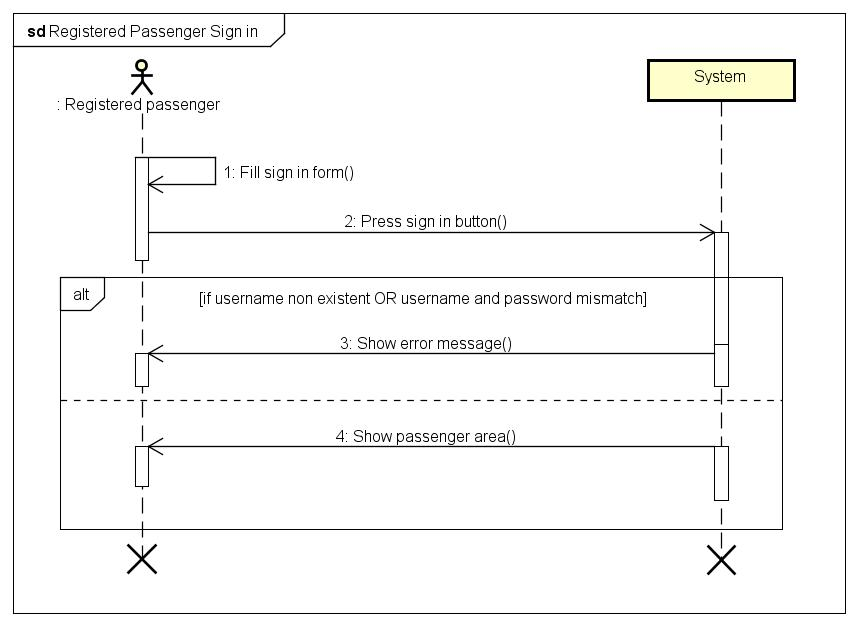
\includegraphics[height=\textheight]{../SE2_SD/RegisteredPassengerSignIn}
		\caption{Sequence Diagram - Registered Passenger Sign In}	
	\end{center}
\end{figure}
\end{landscape}
\newpage
\paragraph{Guest Taxi Request}
\begin{center}
	\begin{tabular}{ | l | p{8cm} |}
		\hline
		Actor &  Guest	\\ \hline
		Preconditions & Nothing		\\ \hline
		Execution Flow & \begin{enumerate}
			\item The guest fills the request form, which requires to insert full name and telephone number and to give position consensus
			\item The guest presses the request button
			\item The system searches and finds an available taxi
			\item The system loads the confirmation request page
		\end{enumerate}		\\ \hline
		Postconditions & The Guest has the code of the taxi he requested	\\ \hline
		Exceptions & GPS position not available; the request fails \\ \hline
	\end{tabular}
\end{center}
\newpage
\begin{landscape}
\begin{figure}[!h]
	\begin{center}			
		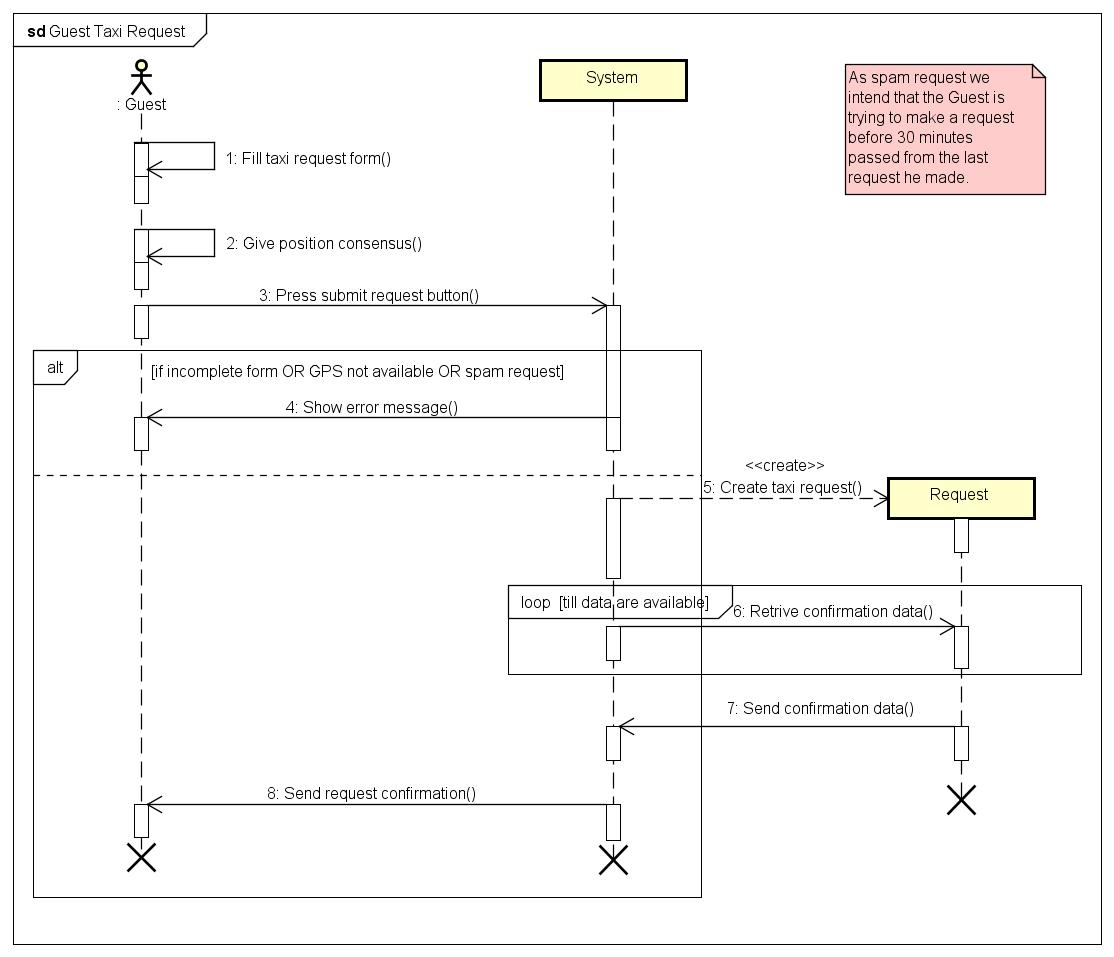
\includegraphics[height=\textheight]{../SE2_SD/GuestTaxiRequest}
		\caption{Sequence Diagram - Guest Taxi Request}	
	\end{center}
\end{figure}
\end{landscape}
\newpage
\paragraph{Registered Passenger Taxi Request}
\begin{center}
	\begin{tabular}{ | l | p{8cm} |}
		\hline
		Actor &  Registered Passenger	\\ \hline
		Preconditions & The registered passenger is registered to the service	\\ \hline
		Execution Flow & \begin{enumerate}
			\item The registered passenger signs in to the service (as written above) and access the Passenger Area page
			\item The registered passenger gives position consensus and presses the request button
			\item The system searches and finds an available taxi
			\item The system loads the confirmation request page
		\end{enumerate}		\\ \hline
		Postconditions & The registered passenger has the code of the taxi he requested	\\ \hline
		Exceptions & GPS position not available; the request fails \\ \hline
	\end{tabular}
\end{center}
\newpage
\begin{landscape}
\begin{figure}[!h]
	\begin{center}			
		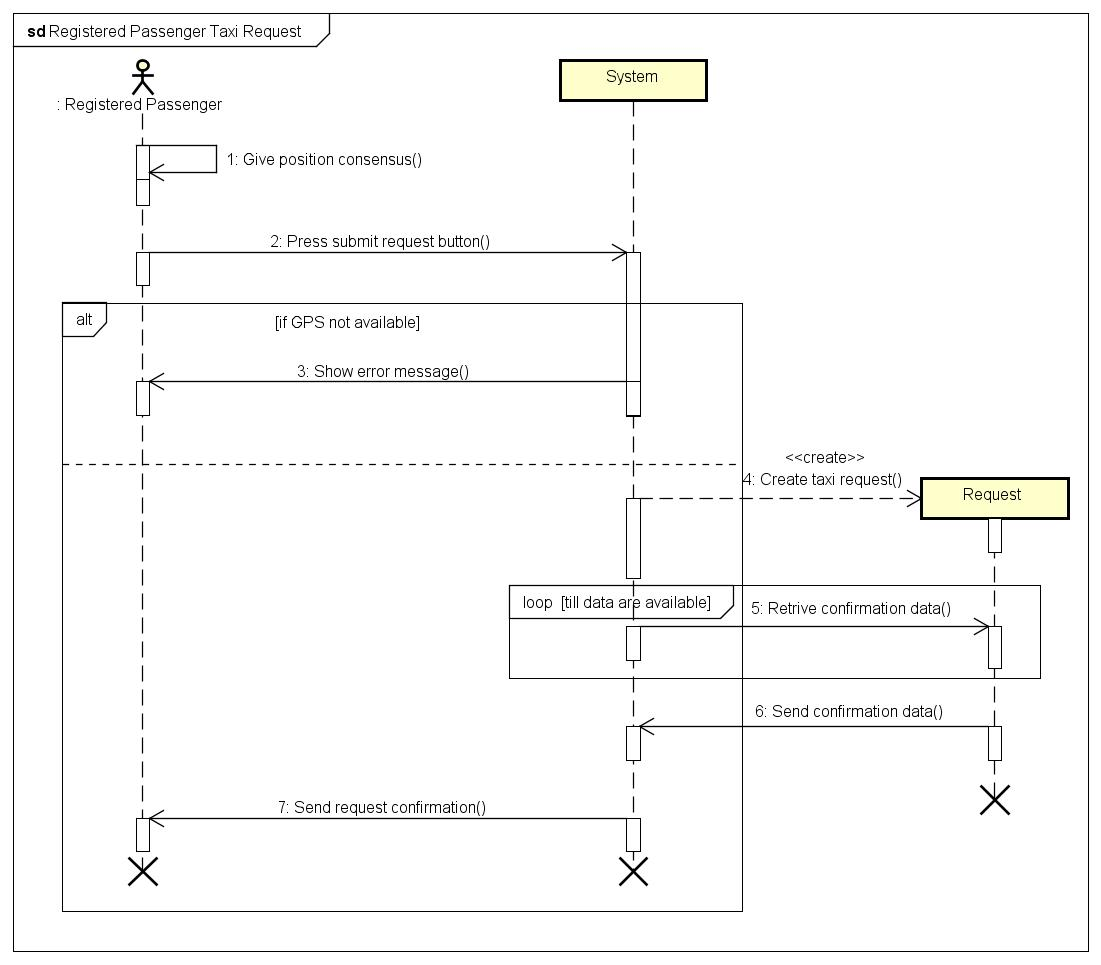
\includegraphics[height=\textheight]{../SE2_SD/RegisteredPassengerTaxiRequest}
		\caption{Sequence Diagram - Registered Passenger Taxi Request}	
	\end{center}
\end{figure}
\end{landscape}
\newpage
\paragraph{Cancel a reservation}
\begin{center}
	\begin{tabular}{ | l | p{8cm} |}
		\hline Actors & Registered passenger
		\\ \hline
		Preconditions &
		The user is logged into the system as registered passenger and has already made
		a reservation
		\\ \hline
		Execution Flow &
		\begin{enumerate}
			\item The user accesses his personal page with the list of reservations
			\item The user selects the reservation that wants to delete and presses the apposite
			button
			\item The system cancels his reservation and reloads the Passenger Area page
		\end{enumerate}
		\\ \hline
		Postconditions & The reservation is cancelled and no requests will be forwarded
		\\ \hline
		Exceptions &
		It's too late to cancel the reservation (after 10 minutes before the time established):
		the reservation is not cancelled and the user is notified.
		\\ \hline
	\end{tabular}
\end{center}
\newpage
\begin{landscape}
\begin{figure}[!h]
	\begin{center}			
		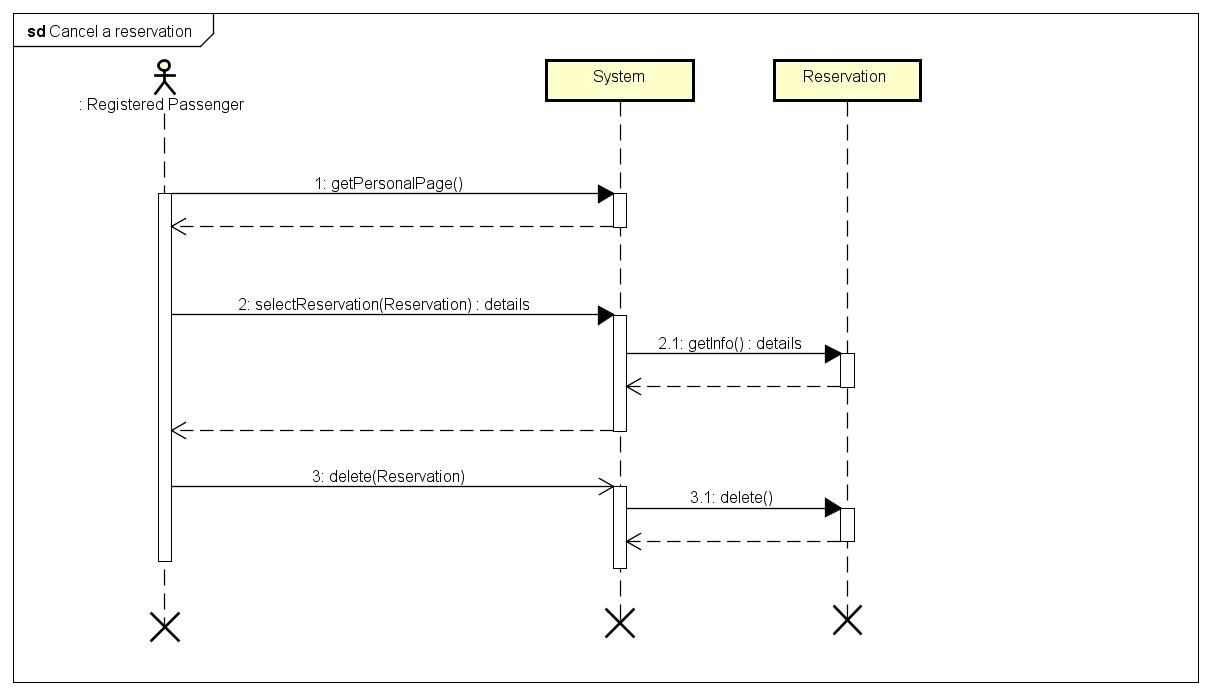
\includegraphics[height=\textheight]{../SE2_SD/CancelAReservation}
		\caption{Sequence Diagram - Registered Passenger Sign In}	
	\end{center}
\end{figure}
\end{landscape}
\newpage
\paragraph{Give availability}
\begin{center}
	\begin{tabular}{ | l | p{8cm} |}
		\hline Actors & Taxi driver
		\\ \hline
		Preconditions &
		The user is logged into the system as taxi driver and is using the mobile application
		\\ \hline
		Execution Flow &
		\begin{enumerate}
			\item The taxi driver accesses his personal area
			\item The taxi driver presses the apposite button
			\item The system sets the taxi driver status as available
			\item The system inserts the taxi driver in his area queue
		\end{enumerate}
		\\ \hline
		Postconditions & 
		The taxi driver is now available and will receive notifications of taxi requests.
		\\ \hline
		Exceptions &
		The taxi driver is already available: the system will not react anyway at the button
		pressure.
		\\ \hline
	\end{tabular}
\end{center}
\newpage
\begin{landscape}
\begin{figure}[!h]
	\begin{center}			
		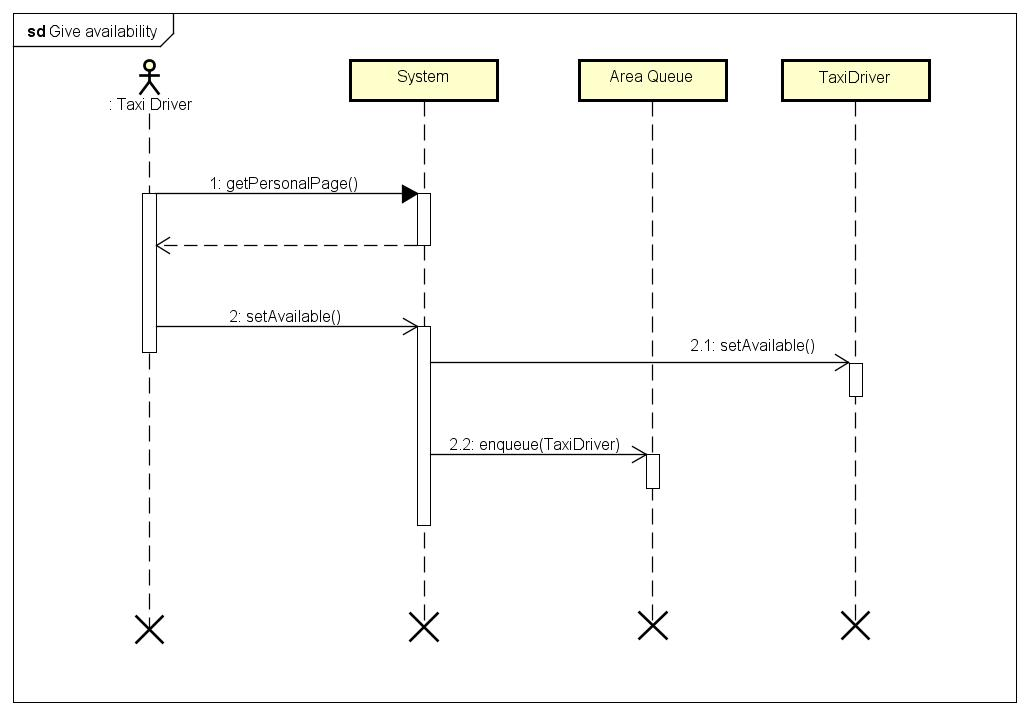
\includegraphics[height=\textheight]{../SE2_SD/GiveAvailability}
		\caption{Sequence Diagram - Registered Passenger Sign In}	
	\end{center}
\end{figure}
\end{landscape}
\newpage
\paragraph{Revoke availability}
\begin{center}
	\begin{tabular}{ | l | p{8cm} |}
		\hline Actors & Taxi driver
		\\ \hline
		Preconditions &
		The user is logged into the system as taxi driver and is using the mobile application
		\\ \hline
		Execution Flow &
		\begin{enumerate}
			\item The taxi driver accesses his personal area
			\item The taxi driver presses the apposite button
			\item The system sets the taxi driver status as unavailable
			\item The system removes the taxi driver from his area queue
		\end{enumerate}
		\\ \hline
		Postconditions & 
		The taxi driver is now unavailable and will not receive notifications of taxi requests.
		\\ \hline
		Exceptions &
		The taxi driver is already unavailable: the system will not react anyway at the button
		pressure.
		\\ \hline
	\end{tabular}
\end{center}
\newpage
\begin{landscape}
\begin{figure}[!h]
	\begin{center}			
		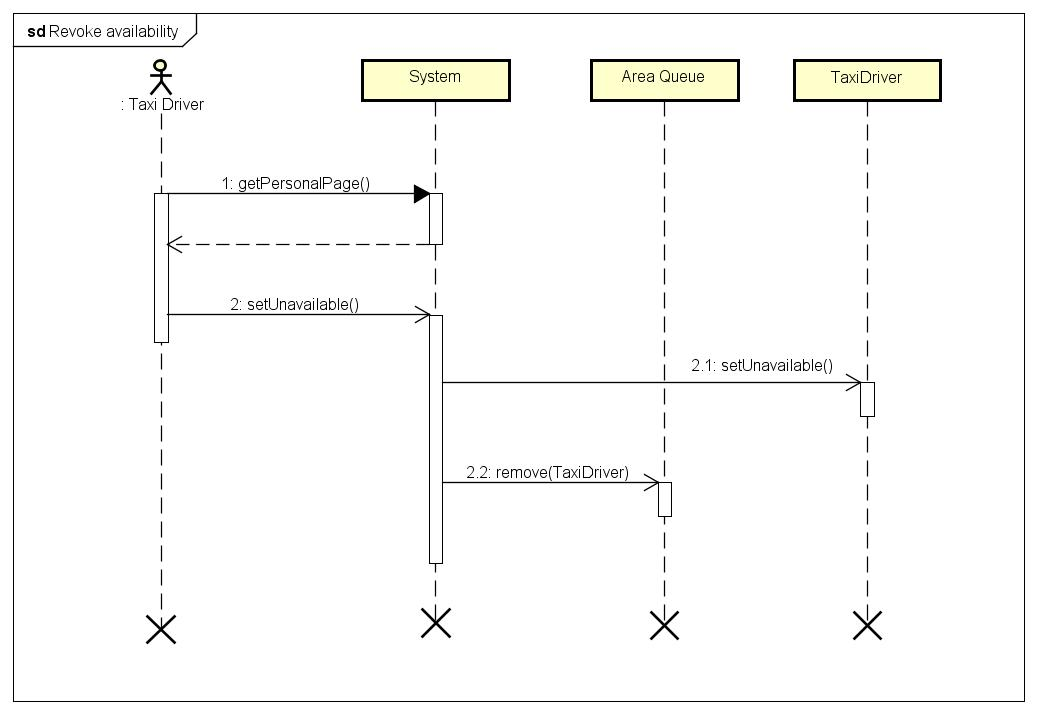
\includegraphics[height=\textheight]{../SE2_SD/RevokeAvailability}
		\caption{Sequence Diagram - Registered Passenger Sign In}	
	\end{center}
\end{figure}
\end{landscape}
\newpage
\paragraph{Accept a ride request}
\begin{center}
	\begin{tabular}{ | l | p{8cm} |}
		\hline Actors & Taxi driver
		\\ \hline
		Preconditions &
		The user is logged into the system as taxi driver and is using the mobile application
		\\ \hline
		Execution Flow &
		\begin{enumerate}
			\item The taxi driver receives the notification of a request
			\item The taxi driver accesses his personal page
			\item The taxi driver presses the Accept button
			\item The system notifies the user who asked for the taxi sending him
			information about the taxi and the arrival time
		\end{enumerate}
		\\ \hline
		Postconditions & The taxi driver is not enqueued again and the user's request
		is considered satisfied
		\\ \hline
		Exceptions &
		The taxi driver does not answer within 1 minute:
		the system automatically records a rejection.
		\\ \hline
	\end{tabular}
\end{center}
\newpage
\begin{landscape}
\begin{figure}[!h]
	\begin{center}			
		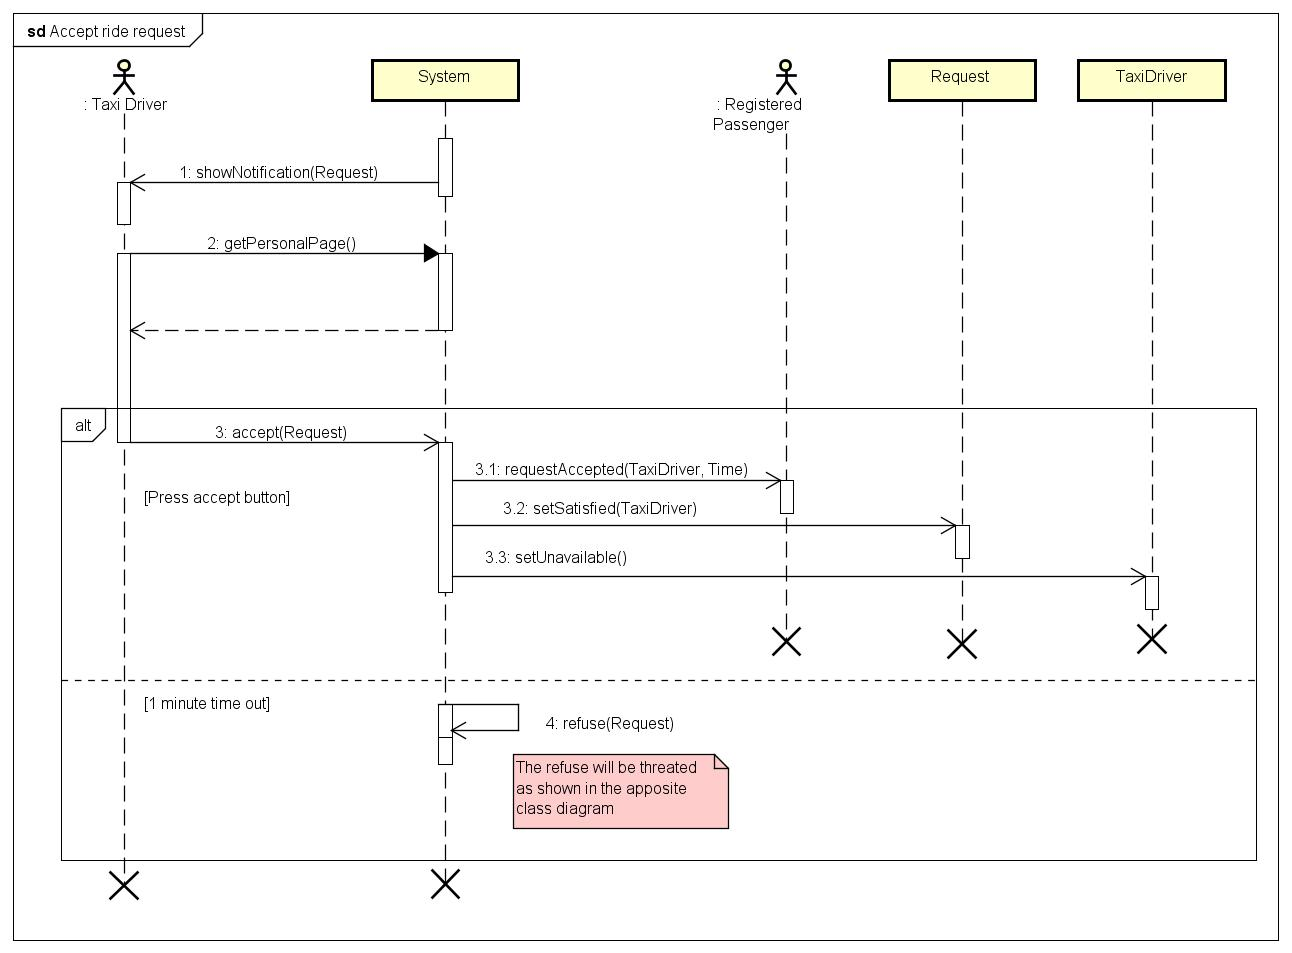
\includegraphics[height=\textheight]{../SE2_SD/AcceptRideRequest}
		\caption{Sequence Diagram - Registered Passenger Sign In}	
	\end{center}
\end{figure}
\end{landscape}
\newpage
\paragraph{Refuse a ride request}
\begin{center}
	\begin{tabular}{ | l | p{8cm} |}
		\hline Actors & Taxi driver
		\\ \hline
		Preconditions &
		The user is logged into the system as taxi driver and is using the mobile application
		\\ \hline
		Execution Flow &
		\begin{enumerate}
			\item The taxi driver receives the notification of a request
			\item The taxi driver accesses his personal page
			\item The taxi driver presses the Decline button
			\item The system records the rejection and reinserts the taxi at the end of
			the area queue
			\item The system sends the request notification to another taxi
		\end{enumerate}
		\\ \hline
		Postconditions & The taxi driver is enqueued again and the user's request
		is considered unsatisfied
		\\ \hline
		Exceptions &
		The taxi driver does not answer within 1 minute:
		the system automatically records a rejection.
		The taxi driver is at the third consecutive rejection:
		the system does not enqueue the taxi driver and sets his status as unavailable
		\\ \hline
	\end{tabular}
\end{center}
\newpage
\begin{landscape}
\begin{figure}[!h]
	\begin{center}			
		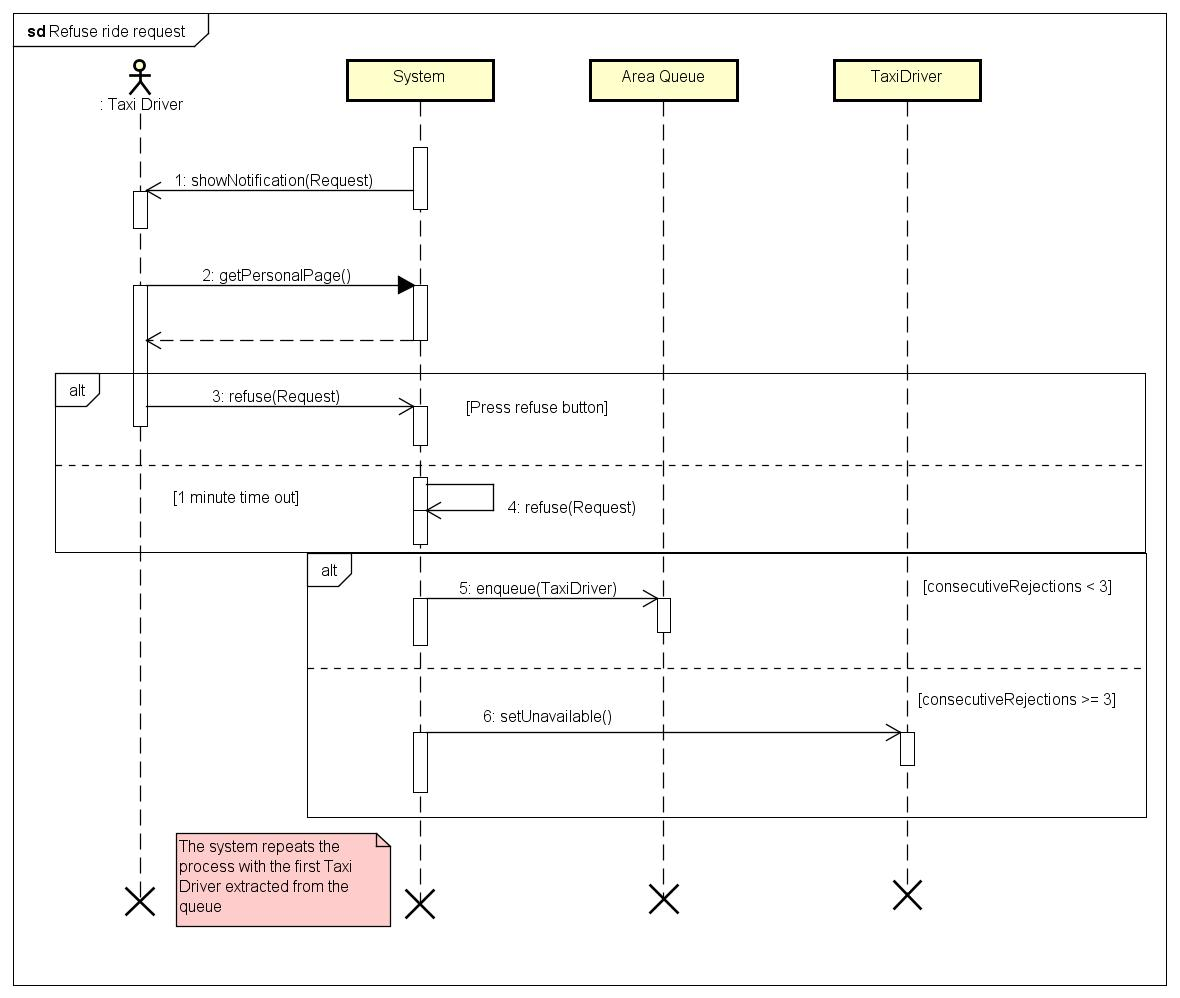
\includegraphics[height=\textheight]{../SE2_SD/RefuseRideRequest}
		\caption{Sequence Diagram - Registered Passenger Sign In}	
	\end{center}
\end{figure}
\end{landscape}
\newpage